 %% Copyright (C) 2019 by
 %%   Robert L. Read <read.robert@gmail.com>, Megan Cadena <megancad@gmail.com>

 %% This program is free software: you can redistribute it and/or modify
 %% it under the terms of the GNU General Public License as published by
 %% the Free Software Foundation, either version 3 of the License, or
 %% (at your option) any later version.

 %% This program is distributed in the hope that it will be useful,
 %% but WITHOUT ANY WARRANTY; without even the implied warranty of
 %% MERCHANTABILITY or FITNESS FOR A PARTICULAR PURPOSE.  See the
 %% GNU General Public License for more details.

 %% You should have received a copy of the GNU General Public License
 %% along with this program.  If not, see <http://www.gnu.org/licenses/>.

\documentclass{article}
\usepackage{hyperref}
\usepackage{amsmath}
\usepackage{amssymb}
\usepackage{mathtools}
\usepackage{draftwatermark}


\SetWatermarkText{DRAFT}
\SetWatermarkScale{6}
\SetWatermarkLightness{0.95}

\title{A Consideration of Inflatable Circles}

\author{Robert L. Read
  \thanks{read.robert@gmail.com}
  email: \href{mailto:read.robert@gmail.com}{read.robert@gmail.com}\\
Megan Cadena
  \thanks{megancad@gmail.com}
  email: \href{mailto:megancad@gmail.com}{megancad@gmail.com}
  }


\begin{document}

\maketitle

\section{Introduction}
This is a study of the basic math of inflatable spheres as a tool for soft robotics.
We begin with a study in two dimension to simplify the problem.
Our final goal is to analyze three dimensional soft robots composed of inflatable
spheres.

\begin{figure}
     \centering
     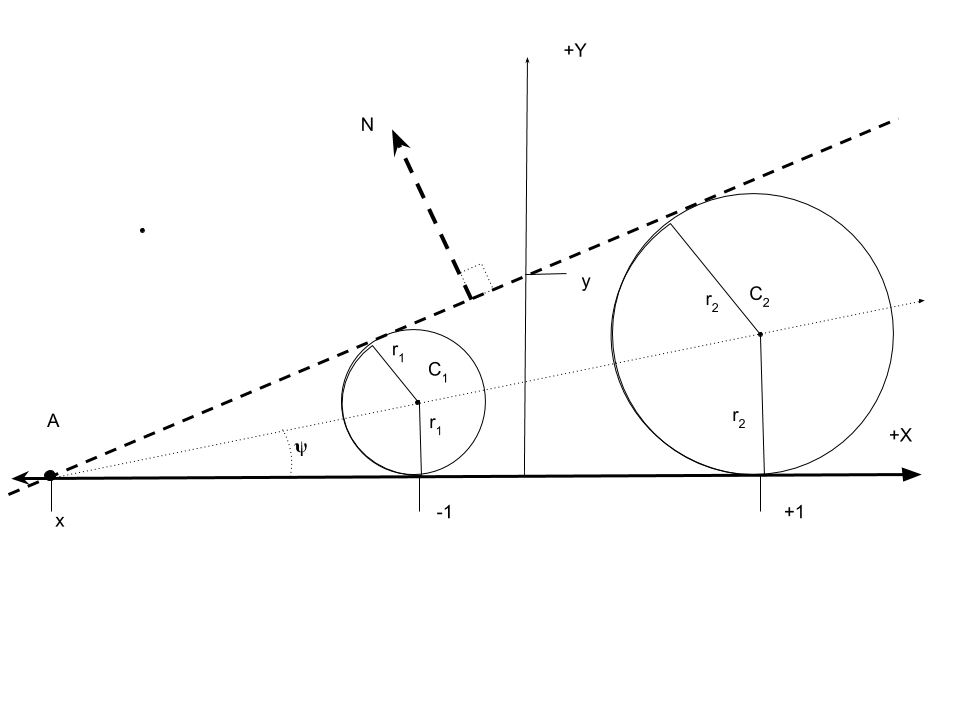
\includegraphics[width=0.80\textwidth]{figures/FixedAxisCircles.png}
     \caption{Problem I: Fixed Circles Centers}
  \label{fig:fixed}
\end{figure}

\section{Problem I: Circles in Fixed Postions}

A very simplified version of the problem is to imagine that a two-dimensional
plane.  Instead of spheres, we will assume we have circles of changable radius.
This is in fact realistic of a soft robot constrained to a plane.




Eventually we hope to have circles pressing against each other, or tangent
or ``kissing''. However, the problem is a bit simpler if we assume we have
two circles, each of which is constrained to have its center on the a vertical
line (see Figure \ref{fig:fixed}.)  We place the circle $C_1$ with radius $r_1$ on the $x = -1$ line, and
assume that it rests on a shelf or plane on the $x$-axis.
Assume the $C_2$ circle whose radius if $r_2$ is on the $x = 1$ line.

Let $A$ the intersection of the tangent line supported
by the inflatable circles with the $x$-axis. Call the distance of $A$
on the $x$-axis $x$. Let $\psi$ be the angle formed by the
circle centers with the $x$ axis (measured counterclockwise).

If the radii are less than $1$ so that no issues of intersection
of the circles arise, we have:

\begin{align}
  \tan{\psi} &= \frac{r_1}{x-1} = \frac{r_2}{x+1}  \\
  r_2(x - 1) &= r_1(x+1) \\
  r_2x - r_2 &= r_1x + r_1 \\
  r_2x - r_1x &= r_1 + r_2 \\
  x(r_2 - r_1) &= r_1 + r_2 \\
  x &= \frac{r_1+r_2}{r_2 - r_1} \\
  \tan{\psi} &= \frac{r_1}{x - 1} \\
  \psi &= \arctan{\frac{r_1}{x - 1}} \\
  N &=  \begin{bmatrix} -\sin{\psi} \\ \cos{\psi}  \end{bmatrix} \\
\end{align}





\section{Problem II: Tangent Circles}



\begin{figure}
     \centering
     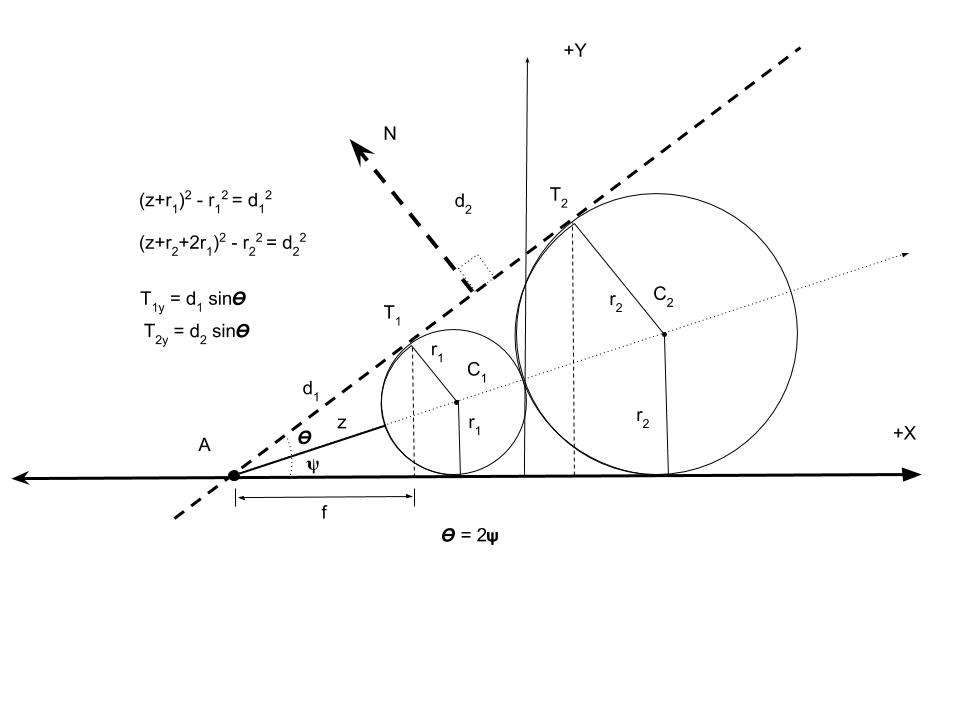
\includegraphics[width=0.80\textwidth]{figures/TangentCirclesGeneral.png}
     \caption{Problem II: Tangent Circles}
  \label{fig:Tangent}
\end{figure}

\begin{align}
\frac{r_2}{||(C2 - A)||} &= \frac{r_1}{||(C_1-A)||} \\
||C2 - A|| &= r_2+2r_1+z \\
||C1 - A|| &= r_1 + z \\
\frac{r_2}{r_2+2r_1+z} &= \frac{r_1}{r_1+z} \\
z &= -\frac{2 r_1^2}{r_1 - r_2} \text{ and } r_1 \neq r_2 \text{ and } r_1 r_2 (r_1 + r_2) \neq 0 \\
\sin{\psi} &= \frac{r_1}{z + r_1} \\
\sin{\psi} &= \frac{r_1}{z + r_1} \\
\theta &=2 \arcsin{\frac{r_1}{z+r_1}} \\
N_x &= -\sin{\pi/2 + \theta} \\
N_y &= -\cos{\pi/2 + \theta} \\
\end{align}

We would like to know the coordinates of $T_1$ and $T_2$.

\begin{align}
  d_1 &= \sqrt{(z+r_1)^2 - r_1^2} \\
  d_2 &= \sqrt{(z+r_2+2r_1)^2 - r_2^2} \\
  T_{1y} &= d_1\sin{\theta} \\
  T_{2y} &= d_2\sin{\theta} \\
  A_x &= (z + 2r_1)\cos{\psi} \\
  f  &= \sqrt{d_1^2 - T_{1y}^2} \\
  T_{1x} &= A_x - f \\
  T_{2x} &=  \sqrt{d_2^2 - T_{2y}^2} - A_x \\
\end{align}


The slope of the vector $\overrightarrow{T_1T_2}$ is $\tan{\theta}$.
  \begin{align}
    \overrightarrow{T_1T_2}_x &= \cos{\theta} \\
    \overrightarrow{T_1T_2}_y &= \sin{\theta}
    \end{align}

  \section{Problem III: Support points of Two tangent spheres }

  In attempting to solve a latter problem, we identified the following problem as useful.

  Suppose that you have two spheres which are tangent. The centers of these spheres are
  in the $XY$-plane, in arbitrary positions.   Find the three-dimensional coordinates
  of the ``support points'', which are the points upon which a flat plane would rest
  if lowered onto the spheres. If the spheres are different sizes, these will not quite
  be the tops of the spheres.  Assume the plane is symmetric about the support line; that
  is, not tilted to one side.



\section{Problem: Three Touching Circles}

Our goal is to be able to determine the orientation of plane resting on top of three spheres of different radii which are touching each
other.
Because there is a plane through any three points and we have three spheres, we can construct the plane through
the center of these points.
The projection of the edges of the spheres onto this plane form three touching circles.
Knowing the position of these circles is a valuable prelude to solving the three dimenstional problem.

\begin{figure}
     \centering
     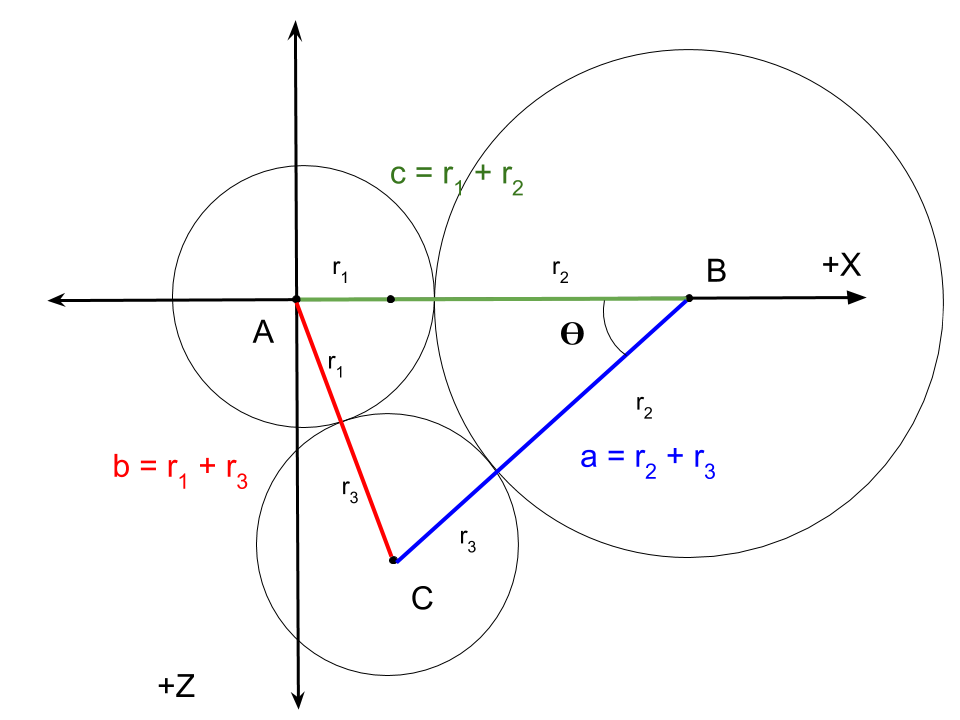
\includegraphics[width=0.80\textwidth]{figures/ThreeTouchingCircles.png}
     \caption{Three Touching Circles}
  \label{fig:Tangent}
\end{figure}

To solve this problem most conveniently, we place the first circle on the negative $x$-axis, and the second circle
on the positive $x$-axis, with the circles intersecting at the origin.
The third circle is place in the positive $y$ direction. It's center will not be on the $y$-axis itself unless the
radii of the first two circles are equal.

We seek a formula for the coordinates of the third circle in terms of three input radii $r_1,r_2,r_3$.

Because the distance between adjacent circles is the sum of their radii, define:
\begin{align}
a  &= r_2 + r_3 \\
b  &= r_1 + r_3 \\
c  &= r_1 + r_2
\end{align}

Then we can use the cosine law to compute the angle $\angle ABC = \theta$:


\begin{align}
  \theta  &= \arccos{\frac{a^2 + b^2 - c^2}{2bc}} \\
  \theta  &= \arccos{\frac{(r_2+r_3)^2 + (r_1+r_3)^2 - (r_1+r_2)^2}{2(r_2+r_3)(r_1+r_3)}} \\
\end{align}

It is clear that once $\theta$ has been calculated:

\begin{align}
 C_y  &= a\sin{\theta}
\end{align}
Allowing us to form a right triangle $\triangle ACD$ and use the Pythagorean theorem:
\begin{align}
  b^2  &= C_y^2 + (r_1-C_x)^2 \\
  b^2 - C_y^2  &= (r_1-C_x)^2  \\
  \sqrt{b^2 - C_y^2}  &= r_1-C_x  \\
  C_x &= r_1 -  \sqrt{b^2 - C_y^2}
\end{align}

\section{A Progression of Problems}

Because we now believe we can model the main problem as the rotation of a plane tangent to a cone about the cone,
there are a number of easier problems which may lead us to a solution:
\begin{enumerate}
\item In 2D, rotate a tangently line to a circle until it is coincient on an outside point.  That is, given the
  center of a circle $C$, a radius $r$, another point $p$, what angular rotation (measured against $x$-axis) gives
  the rotation that makes a line tangent to $C$ touch $p$?
\item Given two spheres, what is the equation for the cone tangent to both?
  \item Is the problem better thought of as the intersection of several spheres?
  \end{enumerate}

\section{Three Touching Spheres}

Note: This problem is mentioned in an advanaced textbook on solid geometry from 1881\cite{payne1881}.

Our fundamental goal now is to describe three touching spheres. As robotocists,
our interest is in the slope of the plane of the tops of these spheres
as if they were resting on a table. Then by inflating or deflating spheres,
we would be able to control the direction of a plane or platform.
Such a device is sometimes called a parallel manipulator, of which a
Stewart Platform\cite{wiki:stewart} (\url{https://en.wikipedia.org/w/index.php?title=Stewart_platform&oldid=898429010})
is the best-known example.

The fundamental action of a parallel manipulator is to tilt a plane or platform in a desired direction.
Having developed the math for the three touching circles in the previous section, we now use it
to find the normal of the a plane resting on the top of three spheres by choosing our
coordinate system to the plane defined by the center points of the three spheres.
In this coordinate system, the $z$-coordinate of the center of all spheres is $0$.
The projection of all three spheres into this plane produces three touching circles.
We seek an expression for the normal of the plane of the tops of these spheres as a function
purely of the three radii. Call this plane the {\em top} plane.

As the top plane tilts, the points tangent to this plane move away from the highest points on each of
the three spheres, making the problem more difficult.

This problem can clearly be solved quickly using numerical methods, because by guessing
a candidate normal to the top plane, it is relatively easy to compute an error function based
on the distance between the closest point on each sphere to the top plane and the top plane.
We would expect an iterative approach to converge very quickly.

Nonetheless we seek an analytic solution.

\begin{figure}
     \centering
     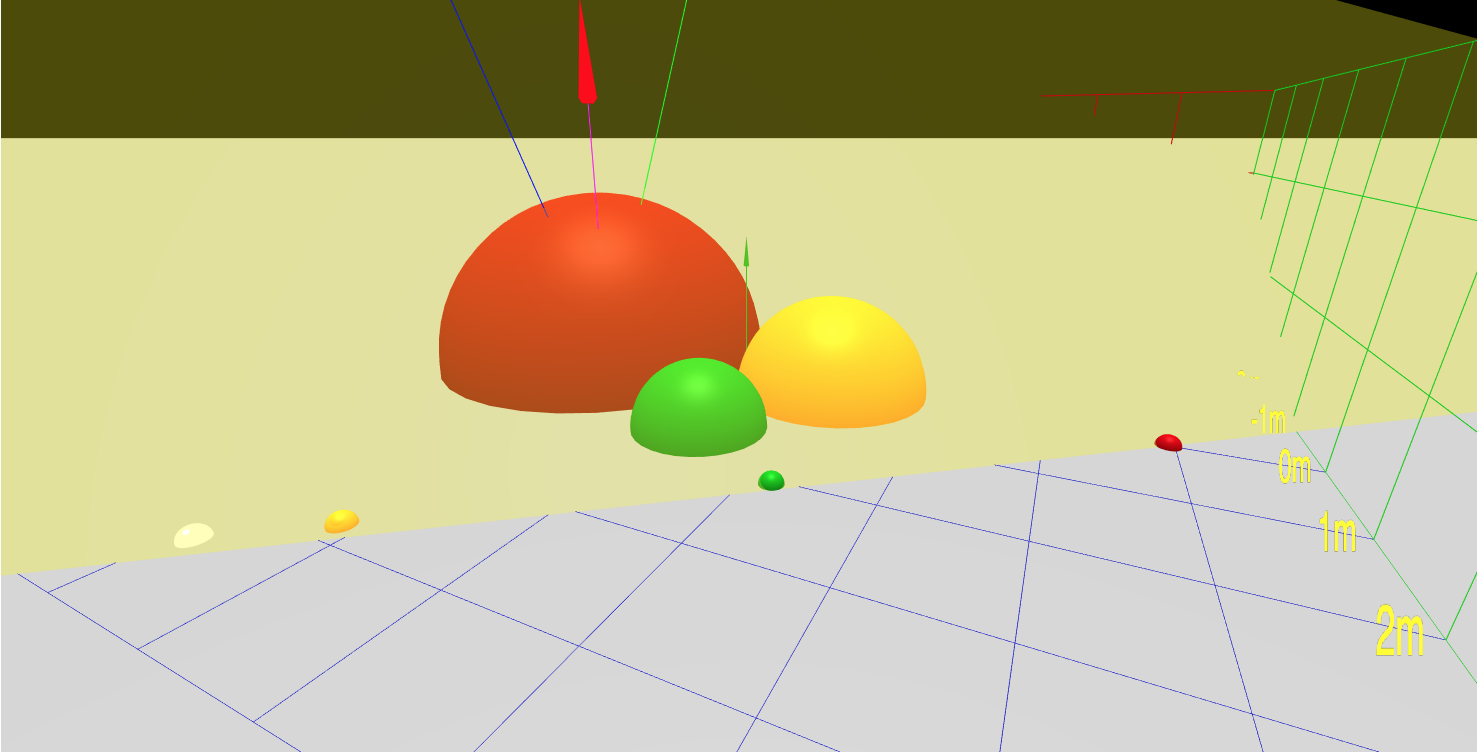
\includegraphics[width=0.80\textwidth]{figures/StandardThreeSphereDiagram.png}
     \caption{Three Touching Spheres}
  \label{fig:fixed}
\end{figure}

\subsection{Variable definitions}

We assume that the spheres centered at points $A,B,$ and $C$
of radii $r_A,r_b,$ and $r_c$. We setup our coordinate system as a right-
handed coordinate system with $XZ$ plane contaning the center of all spheres.
The $A$ sphere is placed at the origin, so that $O = A$, and the $B$ sphere
is place on the positive $X$ axis. Without loss of generality assume $r_a \geq r_b \geq r_c$.
Following computer graphics convention, we think of the $Y$ dimension as vertical.

Taking any two spheres defines a cone whose apex is in the $XZ$ plane.
Call the apex of the $AB$ cone $U$, the $AC$ cone $V$, and the $BC$ cone $W$.

We assert that these three points form a line, which we call the {\em apex line}, in the $XZ$ plane and that this
line is the intersection of the {\em tangent plane} touching all three spheres at a single point
with the $XZ$ plane. We will use points $U$ and $V$ in our calculation.
Let $\alpha$ be the half-angle of the $AB$ cone.

It behooves us to name the intersection of the apex line with the $Z$ axis, $I_z$, so
that we can use it in calculations.

\subsection{Strategy}

We seek to compute the normal of the tangent plane.
Observe that this plane is tangent to all three cones.
Observe that the $AB$ cone intersects
the $A$ sphere in a circle on the surface of the $A$ perpendicular to and centered on the $X$ axis.

A vector of length $r_A$ that begins pointing in the $X$ direction and is rotated counterclockwise
about the $Z$-axis by $\pi/2 - \alpha$.

However, we must rotate this vector about the $X$ axis by an unknown amount $\theta$ in order
to bring capture the tilt which is not purely a rotation about the $Z$ axis.
Since this angle is computed in the $ZY$ plane, we compute a projection of the point $V$ into
that plane, forming a triangle in the $ZY$ plane.  Call this point $I_z$, the intersection
of the apex line with the $Z$-axis.

\begin{align}
 \phi &= \arcsin{\frac{r_c}{I_z}}\\
\theta &= \frac{\pi}{2} - (\frac{\pi}{2} - \phi)\\
\theta &= \phi\\
I_z &= U_x(\frac{V_z}{(U_x - V_x})
\end{align}



\section{Thing to Research}

Idea: It may be possible to solve for the support points as the intersection of cones\cite{shene1994lower}.

Note problem CXLVIII (148). Page 195
Joseph Payne (of the Charterhouse)
``Practical solid geometry; or, Orthographic and Isometric projection.

http://www.coe.org/p/fo/et/thread=11194

https://math.stackexchange.com/questions/2101056/how-to-compute-the-formula-of-common-tangent-plane-of-three-spheres

https://math.stackexchange.com/questions/1129402/solving-a-common-tangent-problem-using-matrices




\bibliographystyle{acm}

\bibliography{softrobotmath}


\end{document}
